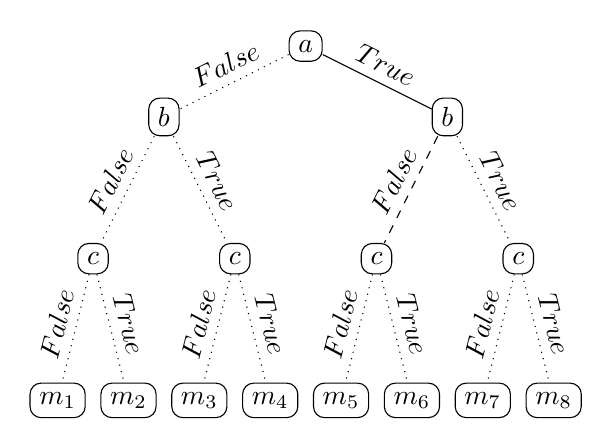
\begin{tikzpicture}[scale=0.9,state/.style={draw, rounded corners, fill=none,text centered, text=black}]
    \node[state] (n1) at (3.5, 5) {$a$};

    \node[state] (n2) at (1.5, 4) {$b$};
    \node[state] (n3) at (5.5, 4) {$b$};
    
    \node[state] (n4) at (0.5, 2) {$c$};
    \node[state] (n5) at (2.5, 2) {$c$};
    \node[state] (n6) at (4.5, 2) {$c$};
    \node[state] (n7) at (6.5, 2) {$c$};

    \node[state] (n8) at (0, 0) {$m_1$};
    \node[state] (n9) at (1, 0) {$m_2$};
    \node[state] (n10) at (2, 0) {$m_3$};
    \node[state] (n11) at (3, 0) {$m_4$};
    \node[state] (n12) at (4, 0) {$m_5$};
    \node[state] (n13) at (5, 0) {$m_6$};
    \node[state] (n14) at (6, 0) {$m_7$};
    \node[state] (n15) at (7, 0) {$m_8$};

    \path[every node/.style={sloped,anchor=south,auto=false}]
        (n1) edge[dotted] node {$False$} (n2)
        (n1) edge node {$True$} (n3)

        (n2) edge[dotted] node {$False$} (n4)
        (n2) edge[dotted] node {$True$} (n5)
        (n3) edge[dashed] node {$False$} (n6)
        (n3) edge[dotted] node {$True$} (n7)

        (n4) edge[dotted] node {$False$} (n8)
        (n4) edge[dotted] node {$True$} (n9)
        (n5) edge[dotted] node {$False$} (n10)
        (n5) edge[dotted] node {$True$} (n11)
        (n6) edge[dotted] node {$False$} (n12)
        (n6) edge[dotted] node {$True$} (n13)
        (n7) edge[dotted] node {$False$} (n14)
        (n7) edge[dotted] node {$True$} (n15);
\end{tikzpicture}
